\chapter{Irish Sign Language}


\section{Introduction}

This chapter provides an overview of the literature on Irish Sign Language. Introducing evolution till nowadays, design features of ISL. Providing an account of how ISL is expressed, specifically how signers use the body to communicate and the issues about it. Moreover, it reviews the features of a natural language in terms of linguistics (phonology and morphology) compared to ISL. 

\section{What is a Sign Language?}

Sign Language is a form of communication used by Deaf and hard-hearing people using visual gesture modality that consists of using body gestures with hands, head, shoulders and facial expressions. \cite{vermeerbergen2023} \\
Sign languages are fully formed and consist of distinct vocabularies and grammatical rules. These languages emerge organically within deaf communities and are not influenced or derived from the spoken languages used in their surroundings.(Vermeerbergen, 1997, 2006; Vermeerbergen et al., 2007; Baker et al., 2016). \\

In the past, sign languages were often overlooked in linguistic research. The primary reason for this disregard was the misconception that sign languages were not genuine natural languages. Many believed all deaf people worldwide used a universal, rudimentary system of gestures and pantomime. Additionally, there was a misconception that sign language involved directly translating the spoken language into signs, aligning the signs with the spoken words in content \cite{vermeerbergen2023}.  

However, neither of these assumptions proved accurate, and their falsehoods gradually began to change after the publication of "Sign Language Structure" by the American linguist Stokoe in 1960. This publication had a significant impact, sparking interest in sign linguistics and leading to a steady increase in recognition. Today, while not all linguists and non-linguists fully acknowledge the linguistic status of sign languages, linguistic research into sign languages has established a solid position within various linguistic subdisciplines. One of Stokoe's contributions was emphasising that the signs used in American Sign Language (ASL) should not be considered as indivisible units but rather as composed of smaller components that distinguish meaning. (Vermeerbergen, Herreweghe, 2023).

While spoken languages use the oral-aural modality, sign languages exploit the visual-gestural modality. As a result, sign languages draw on their specific linguistic mechanisms (Meier, 2002). Signers use visible articulators to communicate: the hands, face, torso and other body parts are needed for communication production, whereas the eyes (and writings, in the case of tactile sign languages used by deafblind people) are required to perceive a signed message. Signs consist of manual and non-manual parameters or building blocks. Manual parameters include hand shape, orientation, movement and location (Baker et al., 2016). Non-manual parameters are movements of the face and body, e.g. mouth gestures and facial expressions (Vermeerbergen, 1997; Baker et al., 2016).

Collectively, the five sign language parameters – shape, Place of Articulation (where the sign is formed), Movement, Orientation (the hand's position about the Place of Articulation), and Non-manual features (body and facial actions) – function in a manner analogous of the components found in spoken languages: cavities, articulators, and features. Although these parameters have different content, they undergo operations that exhibit resemblances to the processes seen in spoken languages, and they are collectively referred to as phonemic feature groups within sign languages. However, it's crucial to recognise that these overarching similarities are tempered by significant differences arising from the influences of modality and iconicity on the system. (Pfau, Steinbach and Woll, 2012) \\
 In the early stages of modern research, the focus on sign languages highlighted the fundamental structural similarities they share with spoken languages. However, recent research has shifted towards recognising systematic typological distinctions (Goldin-Meadow and Brentari 2017 provide a comprehensive overview of this evolving research emphasis). These differences primarily emerge from the interplay between language structure and modality. Phonological and morphological arrangements vary due to sign languages' stronger connection between form and meaning (iconicity or visual motivation) than spoken languages. Sign languages also leverage the characteristics of their articulators (the hands being the primary ones, alongside non-manual articulators like the torso, head, face, eyes, and mouth) and the distinctive attributes of visual and auditory perceptual systems. This space utilisation serves grammatical and discourse functions, resulting in syntactic structures characterised by extensive simultaneity, while spoken languages tend to favour linearity and affixation processes. (Woll, 2023)\\


 \subsection{Sign language phonology}

 Phonetics is the field of study that focuses on speech sounds produced by humans and the organs involved in their production. Phoneticians investigate the process of combining speech sounds to form words and how these sounds interact during speech. Also, phoneticians ask questions such as: How many different sounds do languages use? How does sound travel through the air? How do the ears register it? How can we measure speech? Phoneticians also work on how to describe any sound precisely. Then, in 1888, a phonetic inventory called the International Phonetic Alphabet (IPA) was created, which contains the sounds of human speech represented by a symbol. The IPA was created using the Roman alphabet to write down the sounds of any spoken language. The IPA has been revised to incorporate the new findings. The latest revision was in 2005. \\

Sandler and Lillo-Martin (2006) define phonology as "the
level of linguistic structure that organises the medium through which language
is transmitted." \\
 In addition, Johnston and Schembri (2007) say that phonology is "the study of how sounds are organised into the words and phrases of different languages. Although phonetics and phonology both
originally referred to the study of sounds in spoken language, they are also
used by sign language researchers to refer to the physical properties of signs
(signed language phonetics) and how signs are created from smaller
formational units (signed language phonology)." \\

 According to Woll (2023), from Stokoe's groundbreaking research on American Sign Language (ASL) in 1960, linguists have perceived signs as complex combinations of concurrent handshape configuration, articulation location, and movement. This encompasses the trajectory through the signing space and the internal joint movements within the hand. Each component is considered phonological because modifying them can create a distinct minimal pair. Consequently, in British Sign Language (BSL), words like AFTERNOON1 and ORDER contrast only in Handshape, while AFTERNOON and NAME2 differ solely in location, and AFTERNOON and TWO-HUNDRED solely in movement1. Since Stokoe's initial framework, there have been significant adjustments, particularly in acknowledging the importance of movement sequences and holds within a sign's structure (Liddell and Johnson 1989). Additionally, it's been proposed that these sublexical parameters resemble features more than phonemes. Nevertheless, despite these developments, Stokoe's model has endured as the foundational depiction of sign language phonology.

 \subsection{Sign language morphology}

 The smallest meaningful units of a language are known as morphemes
(Bloomfield, 1933). Morphemes are used in the language to create the larger
units we call words and signs and modify existing terms and gestures.\\

Research conducted crosslinguistic on sign languages from 1970 has discovered that these languages exhibit a simultaneous morphological structure and share similar grammatical categories. Additionally, sign language morphology has two different types: simultaneous and sequential (Aronof, Meir and Sandler, 2012). 

Words within a language are tasked with multiple functions. They serve as tools for language users to denote any concept they wish to communicate, whether it's an object, a thought, an occurrence, or a characteristic. Additionally, words need to interact with one another, enabling users to communicate information by expressing opinions, descriptions, or details about specific subjects or individuals. To accomplish the initial objective, it's essential to establish methods for generating fresh words when denoting novel concepts is necessary. As for the secondary objective, when merged to shape more extensive constructs, words must be capable of undertaking diverse functions like serving as subjects, predicates, or modifiers. Certain words could be tailored for specific roles, and languages might incorporate mechanisms for crafting words for particular functions. (Pfau, Steinbach and Woll, 2012)\\

Sign languages possess words, standardised entities of form-meaning connection akin to spoken languages. These entities hold cognitive significance for their users (Zeshan 2002). They consist of smaller linguistic components and exhibit a dual pattern structure (Stokoe 1960). They demonstrate particular phonological arrangements and are influenced by specific phonological limitations (Sandler 1999; consult Chapter 3, Phonology). Typically, these words in sign language are denoted as "signs."

Three indications propose reasons for the valuable insights that sign language morphology can provide into the mechanics of the grammatical system. Firstly, an inherent iconic foundation is present in all natural sign languages. The second significant aspect is the many methods employed to create intricate words within these languages. Lastly, universal principles governing organisation and structure, which impact spoken language morphology, also sway sign language despite its iconic origin. Thus, morphology is the apparent intersection where iconically driven sign language forms meet linguistic structuring.(Sandler and Lillo-Martin, 2006) \\

Two prevalent, if not universally present, characteristics of sign language morphology include a substantial employment of compounding, whether sequentially or simultaneously, and a diverse array of inflexion types involving modifications in position, speed, repetition, and non-manual attributes. Many sign languages exhibit a considerable degree of inflexion (Zeshan 2003; Sandler and Lillo-Martin 2006; Lutalo-Kiingi 2014), with instances where complete sentences are constructed from a single, highly inflected sign. Signs can undergo inflexion to indicate grammatical aspects such as a person, number, location, aspect, manner, and mood, contingent upon the sign's category (Sutton-Spence and Woll 1999).\\

Sign language morphology often becomes evident by blending meaningful handshapes, positions, and motions. In the context of derivational morphology, handshape alterations can represent numerical values. For instance, within BSL, expressions like "N weeks," "N o'clock," and "N years old" are formed using standardised patterns of location and movement, with the handshape conveying the specific number (Woll and Sutton-Spence, 2023). 


\section{Evolution of Irish Sign Language}

 The history of Irish Sign Language relates to Deaf education and educational policy (Leeson and Saeed,2012). The first recorded school for deaf students in Ireland was founded in 1816. Over the years, various educational institutions were established, including the Claremont Institute, which initially taught a Protestant doctrine but later shifted with the advent of Catholic institutions. In 1846, the Catholic Institution for the Education of the Deaf and Dumb was established, inspired by a similar institution in France (Leeson and Saeed, 2012). The Dominican Sisters managed St Mary's School for Deaf Girls and adapted the French methodical signing system for English teaching. In 1849, the Christian Brothers opened a school for Deaf boys. St Joseph's School in Cabra became the last major institution for Deaf education in the 19th century (McDonnell 1979). On the 20th century, Mary Immaculate School for Deaf Children (Beechpark School) was established in 1956 following a request from Archbishop Charles McQuaid (Matthews 1996b).\\

\subsection{What is Irish Sign Language?}

Irish Sign Language is a visual-gestural language using the signer's hands, torso, face, head, shoulders and eyes. The signs are expressed in the three-dimensional space known as 'signing space'. See Figure 2.1. (Leeson and Saeed, 2012) \\

Irish Sign Language (ISL) is used by an estimated 5,000 Deaf people in the Republic of Ireland and some 1,500 signers in Northern Ireland. It is neither Irish (Gaeilge) on the hands nor English in manual form. (Leeson and Saeed, 2012)

According to Lesson and Saeed (2012), The critical universal features across languages include arbitrariness, iconicity, the duality of articulation, semanticity, creativity, and structural dependence. Leeson and Saeed (2012) say that the arbitrariness of the sign is a feature that receives a lot of attention in the literature. Arbitrariness suggests no necessary link between the word and the object it denotes. Iconicity is about the relationship between the form of the sign and the referent it refers to.
\\
Duality of articulation is the organisation of language at two levels, meaningless or meaningful units. For example, phonemes are typically useless in isolation but are significant when combined as morphemes. For example, indicative signs in ISL must comprise a handshape, a location, a movement and an orientation. Without these combined, we have phonological components of characters but not meaningful morphemes. Thus, a handshape or a place by itself is simply phonetic. Semanticity denotes the use of symbols that refer to objects and actions. For example, the literal sign BOIL is expressed in neutral space in ISL. At the same time, the idiomatic expression BOIL+c (I'm boiling (angry)) consists of the same manual sign BOIL, with one modification: the place of articulation moves from neutral space to the signer's body (stomach area). 
\\
Now terms of creativity in a linguistic sense refers to our capacity to produce and understand an indefinite number of sentences, our ability to create from finite means (for example, a limited number of sounds/handshapes that are possible in a language, a finite pattern of rules, etc.) and an infinite number of utterances. Irish Sign Language is a language that is evolving, and as such, as new themes become relevant to daily life, signs are developed to express new concepts. (Leeson, Saeed, 2012)
\\
Yet another feature of human language is structural dependence: language is arranged in structured chunks, not simple linear sequences. This impacts word order issues, on the one hand, and how we interpret broader lines of meaning, on the other (for example, the scope of negation marking or the identification of a topic). (Leeson, Saeed, 2012)


\section{Phonology of ISL}

In signed languages, phonology focuses on analysing and breaking down the continuous movements of the signer's hands, body, and facial expressions. Specific elements like handshapes are extracted from this gestural flow through phonetic analysis, identifying their linguistic significance. There is no consensus on the inventory of a phonetic alphabet for ISL. For instance, Ó Baoill and Matthews (2000) have identified sixty-six handshapes. See fig. \\
Describing the phonology of a signed language involves exploring
how phonological units are formed by combining handshapes
and other phonetic features and trying to discover the rules that govern how
these units are combined to form higher-level elements like words. (Leeson, Saaed, 2012) \\

The most significant research work in sign languages was made by Stokoe in 1960 in his research paper, where Stokoe used linguistic principles to analyse ASL and identified that it is composed of three main linguistic components: hand configurations, movements, and placement. This analysis of sign language structure laid the foundation for recognising sign languages as real languages.\\

In addition, Battison (1978) suggested adding a parameter of orientation, 
the spatial relationship of the palm and fingers to the signer's body.\\

\subsection{Manual Features} 

The first works in sign language phonology where were described the parameters of the signs, such as hand configuration,
movement, and place of articulation (Stokoe 1960; Stokoe et al. 1965; Klima
and Bellugi 1979).

The manual features consist of Handshape, which pertains to how the hand or hands are configured. Location refers to the placement of the hands concerning the signer's body or the signing space. Movement involves the hands and arms' paths while signing and may encompass internal finger and thumb movements. The orientation of the palm plays a crucial role in phonology and can result in minimal pairs (Leeson and Saaed, 2012).

\subsubsection{Location}

Stokoe (1960) called the parameter location a tab, and he defined a set of members named primes, where location primes include face, nose, and trunk. 
According to research on British Sign Language, Brennan et al. (1984) identify five distinct spatial locations: the head (including the neck), the trunk, the arms, the hands and the area in front of the signer's body. They subdivide each location into specific tabs. For example, the head area is reported to have ten tabs, and each is allocated because certain signs differ only in their position on or near the head. So, in BSL, the eye, ear, nose, mouth and forehead are considered separate tabs. Sandler (1989) introduced the idea of utilising setting features to precisely define specific positions within the primary place of articulation. Per her proposal, these setting features can represent the movements occurring within these central articulatory locations.

ISL has the exact spatial locations as BSL, identifying minimal pairs based on tab differences.

\subsubsection{Handshapes}

A handshape is one of the manual features used to articulate a sign. Handshapes can be said to represent one of the phonetic possibilities of a signed language, and the use of particular handshapes is linguistically determined (Leeson and Saaed, 2012). \\
However, the human hand can adopt an extensive range of alternative forms. It can be clenched into a fist or stretched with fingers spread apart or touching. The writing is flexible at the wrist, allowing the fingers to flex at the knuckles or joints. The thumb can be extended, aligned with the fingers, placed across the palm, or within a closed fist. The index, middle, ring, and little fingers may be extended, curved, or positioned in contact with one another. As we will explore further, despite the multitude of potential hand configurations that can be generated, each specific sign language tends to employ only a limited set of handshapes to construct signs in its core vocabulary. (Johnston and Schembri, 2007)

The size of the handshape inventory may differ from one sign language to another, but there.
There is not as much variation as in the sound inventories of spoken languages.
The study of many sign languages has resulted in lists of frequently occurring handshapes (Baker, 2016).

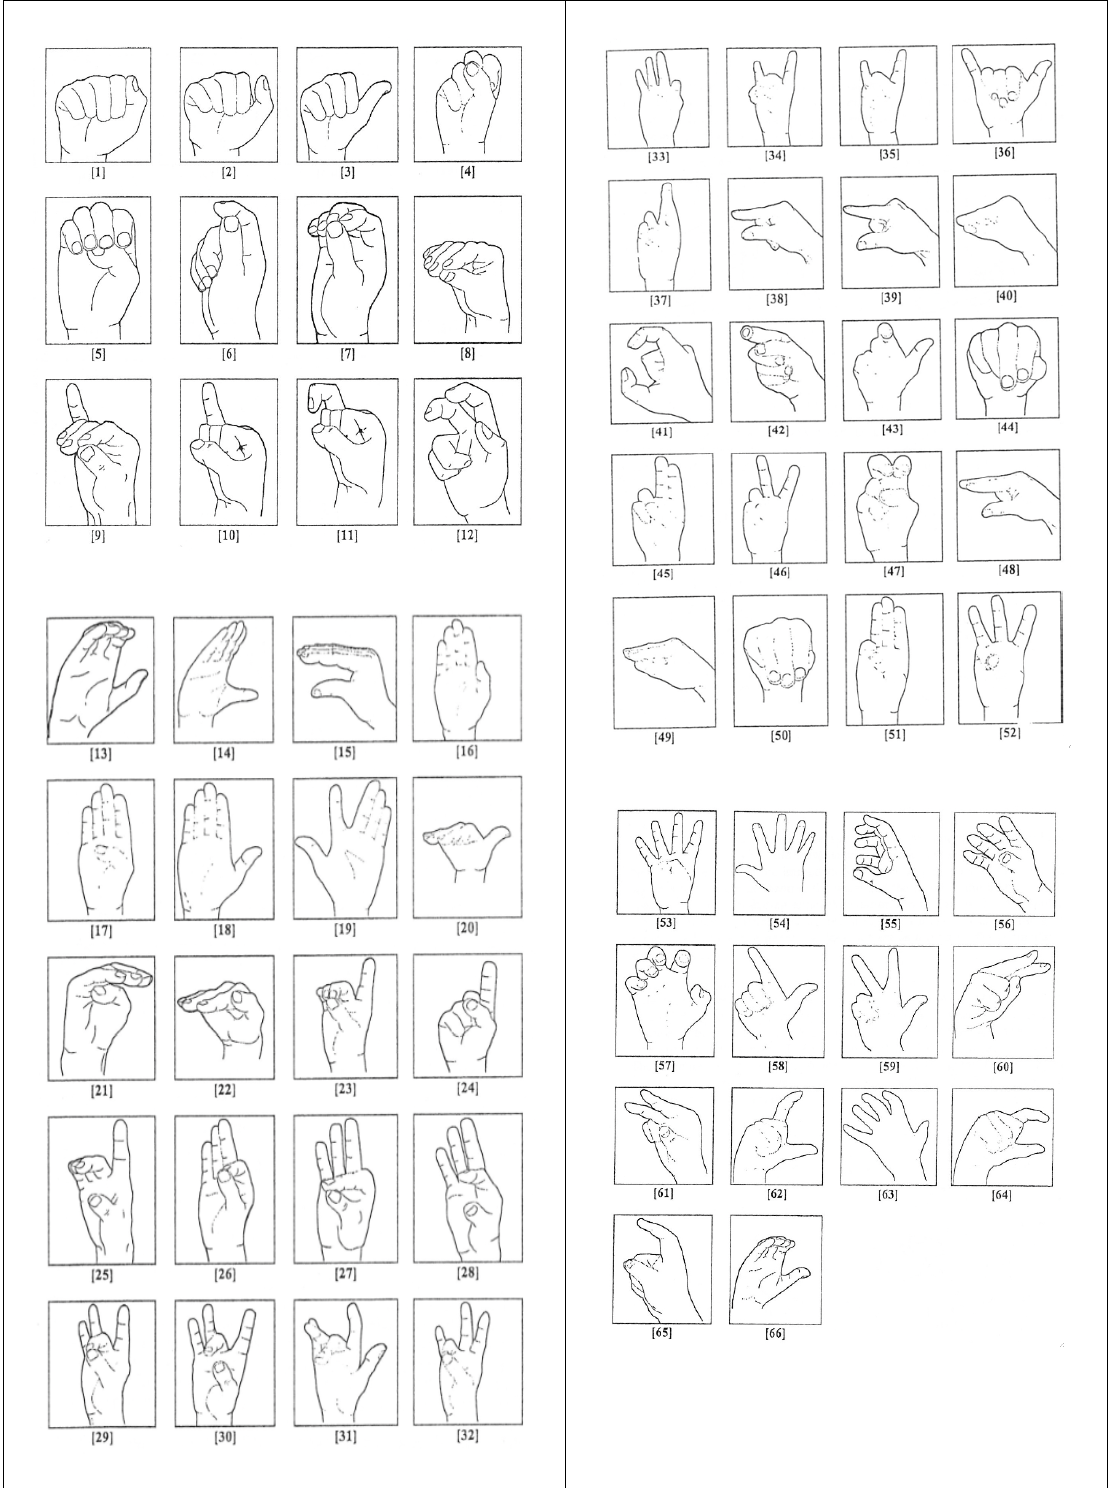
\includegraphics[width=\textwidth]{figures/handshapes.png}

\subsubsection{Movement}

Among the three fundamental components, movement emerges as possibly the most intricate. The hand can traverse away from the body, towards it, upwards, downwards, back and forth, in curved paths like arcs, circles, or spirals. Hand-shape alterations or adjustments in the palm and fingers' orientation could occur. While certain signs employ straightforward motions, others may manifest as intricate amalgamations of diverse movement patterns. If the sign is executed with the palm of the dominant hand positioned toward the signer, additional factors such as the tempo, duration, repetition rate, stress, and the manner of sign production come into play in shaping signs in Auslan (Johnston, 1989a). \\

The feature analysis of movement offered by Friedman (1977) includes four fundamental features: interaction, contact, direction and manner. Also, according to Baker (2016), movement has been considered one of the phonological parameters since Stokoe's phonological description of ASL. There are two types of movements: path and local. The first is the movements of the entire hand. The latter are the movements of the fingers and the wrist (hand-internal movements and orientation changes) 


\subsubsection{Orientation}

Initially, there was a heated debate regarding whether orientation should be considered a fundamental parameter for description. In 1977, Friedman advocated for its inclusion, suggesting that exposure should be defined for each handshape to determine the hand direction of the body. On the other hand, in 1978, Stokoe argued against its necessity. However, Brennan et al. (1984) decided to include the orientation parameter in their analysis based on two key factors. First, orientation can be the sole distinguishing feature between two lexical signs. Second, previous transcription systems that excluded orientation were proven inadequate.
Sandler (1989) proposed categorising the orientation parameter within a node termed 'hand configuration,' referred to as an articulator by Hulst and Kooij (2021). This categorisation was inspired by assimilation patterns observed in lexicalised compounds within both ASL and Israeli Sign Language (ISL), as earlier demonstrated by Sandler in 1987. These patterns revealed that orientation could propagate independently or combine with the overall handshape.

In Irish Sign Language, orientation is crucial in distinguishing between different sets of minimal pairs—for example, the following image (Leeson and Saeed, 2012).

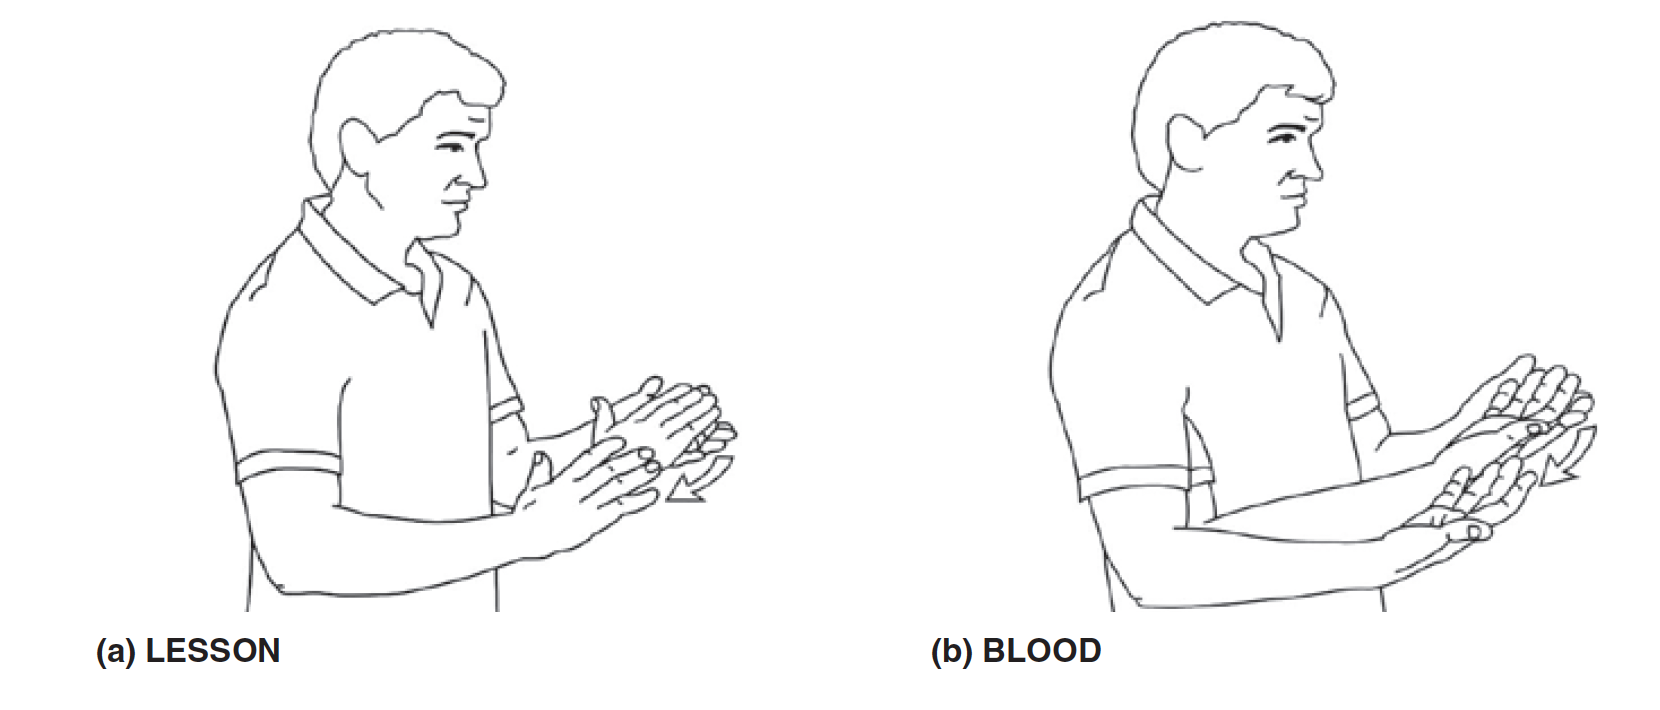
\includegraphics[width=\textwidth]{figures/orientation.png}


\subsection{Non-manual features}

Research on sign languages has revealed the contribution to the meaning of non-manual markers such as facial expressions, head movements, bodily posture and mouthing. 

In signed languages, non-manual signs involve eye, head, body movements, facial expressions, lip movements, and mouth gestures (Johnston and Schembri, 2007).

Mouthings are derived from a spoken language and are evidence of the contact between English and Irish Sign Language. 
Mouth gestures, \textcite{sutton2007mouthings} points out that these are idiomatic gestures of the mouth and cannot be traced back to a spoken language. 

The types of non-manual features used by ISL signers are given in Figure 2.1.

According to \textcite{sutton2007mouthings}, although we commonly associate signed languages with manual communication, they convey crucial linguistic information through non-manual channels, such as the mouth. Studies on sign languages have demonstrated the significance of non-manual elements like facial expressions, head movements, body posture, and mouthing in contributing to the overall meaning of the signed messages.

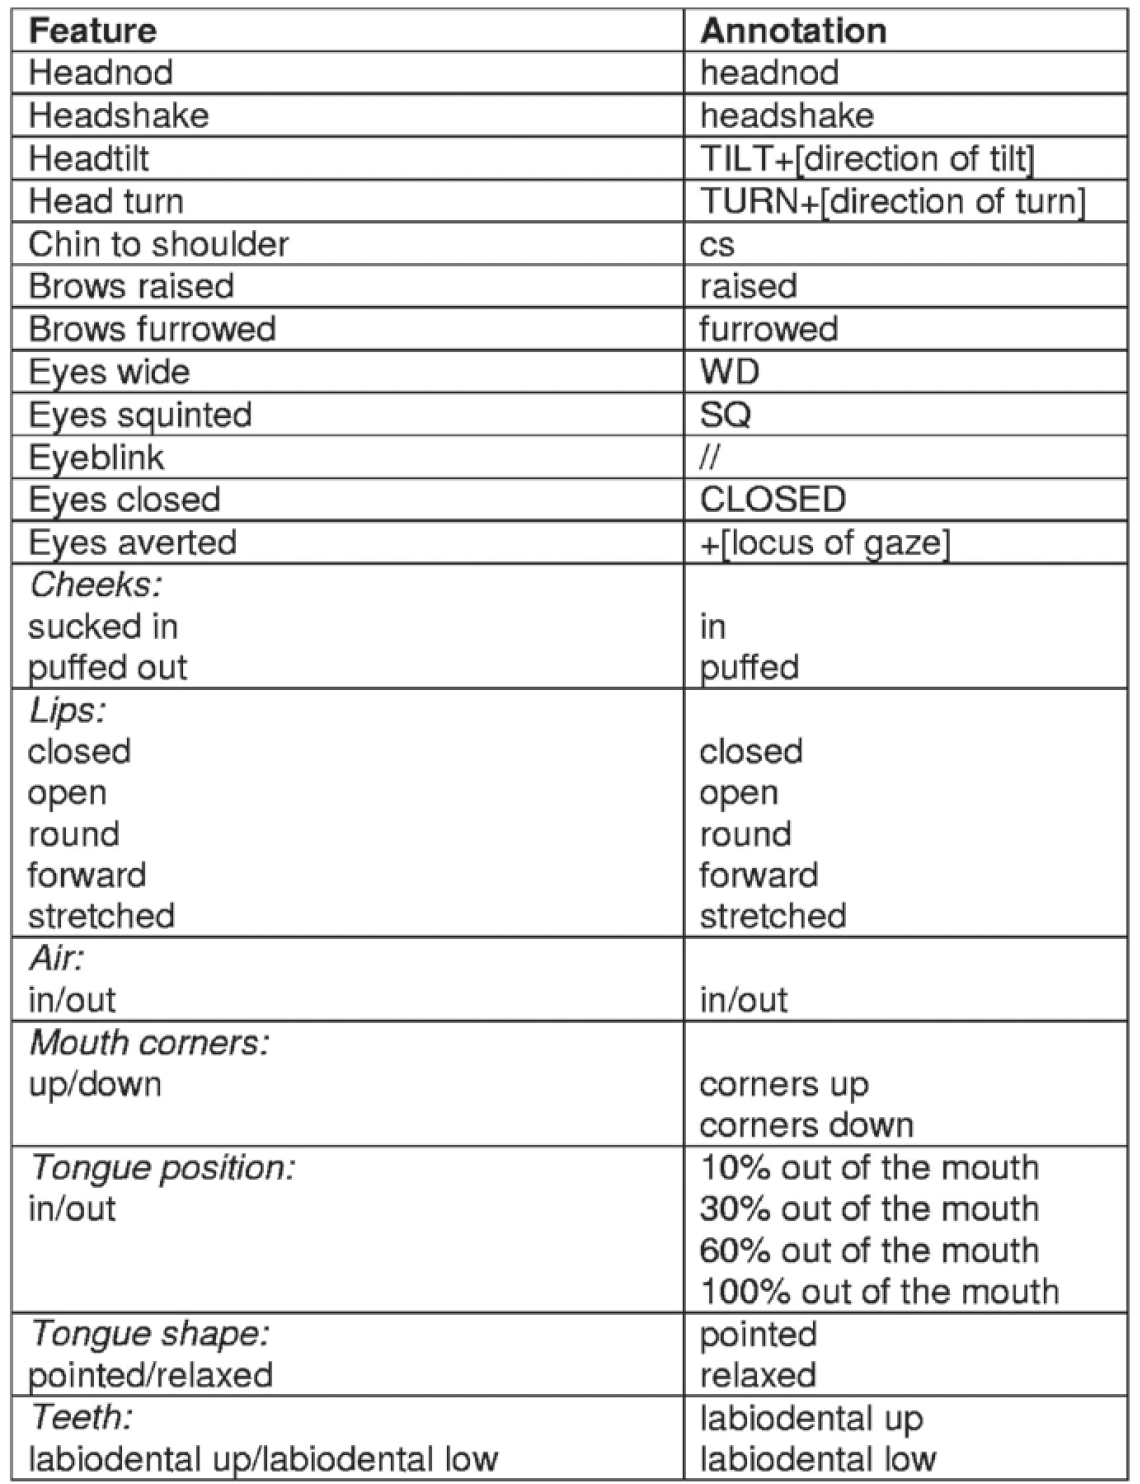
\includegraphics[width=\textwidth]{figures/nm.png}
\captionof{figure}{Extracted from \parencite{leeson2012}:80 Section 4.6, Articulatory descriptors for non-manual features in Irish Sign Language}


\section{Morphology of ISL}

\subsubsection{Morphemes}

As Bloomfield (1933) described, a morpheme is the most elementary meaningful entity within a language. These are the meaningful components of a word that cannot be broken down any further without losing their significance.

Morphemes like bikes and shoes are considered to be 'free morphemes'. In contrast, morphemes like –s (in shoes), -er (in biker) and -ing (ingoing) cannot stand alone as words, but they also carry meaning. Units like these are called 'bound morphemes'. Signed languages also exhibit free and bound morphemes. For example, ISL morphemes function as words in their own right, like HOUSE, GIRL, SISTER and HAVE. (Leeson, Saeed, 2012) \\
Leeson and Saeed follow Brenan in using the term 'word' in a general sense to incorporate spoken, signed and written language. We will use the term 'sign' when referring only to signed languages, considering that 'signs' are equivalent to 'words' in terms of grammatical role. 


\subsubsection{Locus}

A locus denotes a designated spatial point where an entity has been established, and this locus serves as a reference point for subsequent mentions within the discourse. Notably, a locus need not be confined to a specific physical location within the signing space; it can also possess a 3-D function, symbolising a spatial position. Signers employ classifier predicates to depict real-world entities, positioning them in relation to one another in a manner that mirrors their real-world configurations, a spatial arrangement commonly known as topographical space (Liddell, 1990). Also, signers can designate an entity by either producing a lexical sign or a classifier at a specific spatial location or initially signing and directing attention through pointing or eye gaze toward a particular area in space. (Emmorey,  1996) 

The employment of syntactic space is to convey non-locative syntactic and semantic information using loci. Within this context, a locus is characterised as a "random, abstract point" within space that serves as a reference for a particular entity without the exact position within the signing space being of significant relevance. (Vermerbergen and Herrewedge, 2023)

In sign languages, certain verb signs are adjusted to spatially indicate the subjects or objects of the verb, which can be categorised into two types: currently present and not. Regarding non-present referents, signers establish specific spatial locations known as loci (Padden, 1988a; Poizner, Klima, and Bellugi, 1987). When a verb agrees with the subject and object, it typically employs the referential space by starting at the locus representing the subject and ending at the locus representing the object. (Sandler and Lillo-Martin, 2006). 


\subsubsection{Compounds} 


A prevalent word-formation process extensively employed in American Sign Language (ASL), ISL and various other sign languages is compounding, as extensively documented in studies such as those by Klima and Bellugi (1979), Bellugi and Newkirk (1981) and Wallin (1983) in the context of Swedish Sign Language.  \\




\section{The ISL Lexicon}


As users of a language, people possess the knowledge of phonological, morphological, and syntactic principles governing their language, in addition to a substantial repository of individual words or signs. This compilation of known words or symbols is called the lexicon, and each word or sign within this compilation is denoted as a lexical item. (Vali and Lucas, 2001)

The lexicon of a particular language comprises a compilation of elements present within the language. These elements are essential for a speaker to be familiar with as they represent arbitrary signs, often displaying unpredictability. While many of these elements consist of individual words, the lexicon encompasses more extensive entities such as idioms and potentially even smaller components like affixes (Aronoff and Anshen, 2001).

Several researchers, notably Padden (1998), Brentari and Padden (2001), who have predominantly focused on American Sign Language (ASL), have postulated a division within the lexicon. According to their proposals, this division comprises two primary components. The initial component encompasses the complete inventory of native sign vocabulary, commonly termed the lexicon. The secondary component, the non-native lexicon, primarily emerges from interactions with the English language. \\

In their Auslan sign language lexicon research, Johnston and Schembri (2009) introduced a fundamental distinction between the native and non-native lexicon. The native lexicon within Auslan comprises signs that have evolved within the framework of Auslan itself, adhering to a predefined set of nativisation constraints. These nativisation constraints encompass various criteria, including conditions related to symmetry, dominance, and a predisposition for signs to be monosyllabic. Non-native forms contain lexical items that take the form of fingerspelled representations of English words. A parallel distinction is drawn by Brentari and Padden (2001) within the context of the ASL lexicon. They define the non-native lexicon as comprising "signs said to be borrowed from English such as initialised signs and loan signs derived from fingerspelling" (ibid.). Consequently, the non-native lexicon encompasses all signs arising from language contact. An alternative term used to describe the core native lexicon of a sign language is the frozen or established lexicon (Johnston and Schembri, 2009)  

After understanding various perspectives regarding the lexicon in diverse sign languages, let's focus on discussing the lexicon, specifically ISL.

Leeson and Saeed (2012) emphasised a crucial conceptual distinction first introduced by Brennan (1992) within the framework of British Sign Language (BSL). This distinction revolves around segmenting the lexicon into two primary facets: the "established" and the "productive" components. 

The lexicon of Irish Sign Language (ISL) undergoes a multifaceted influence from various sources. These encompass lexical borrowings drawn from British Sign Language (BSL) and French Sign Language, in addition to influences stemming from the English language through mechanisms such as mouthed, initialised, fingerspelled, and Cued Speech elements. Furthermore, the lexicon is subject to gestural components, such as gestures associated with object manipulation, which can be regarded as substrates contributing to the lexicalisation of certain signs. ISL presents free and bound morphemes within its linguistic structure like other sign languages. (Leeson, Saeed, and Grehan, 2015)\\


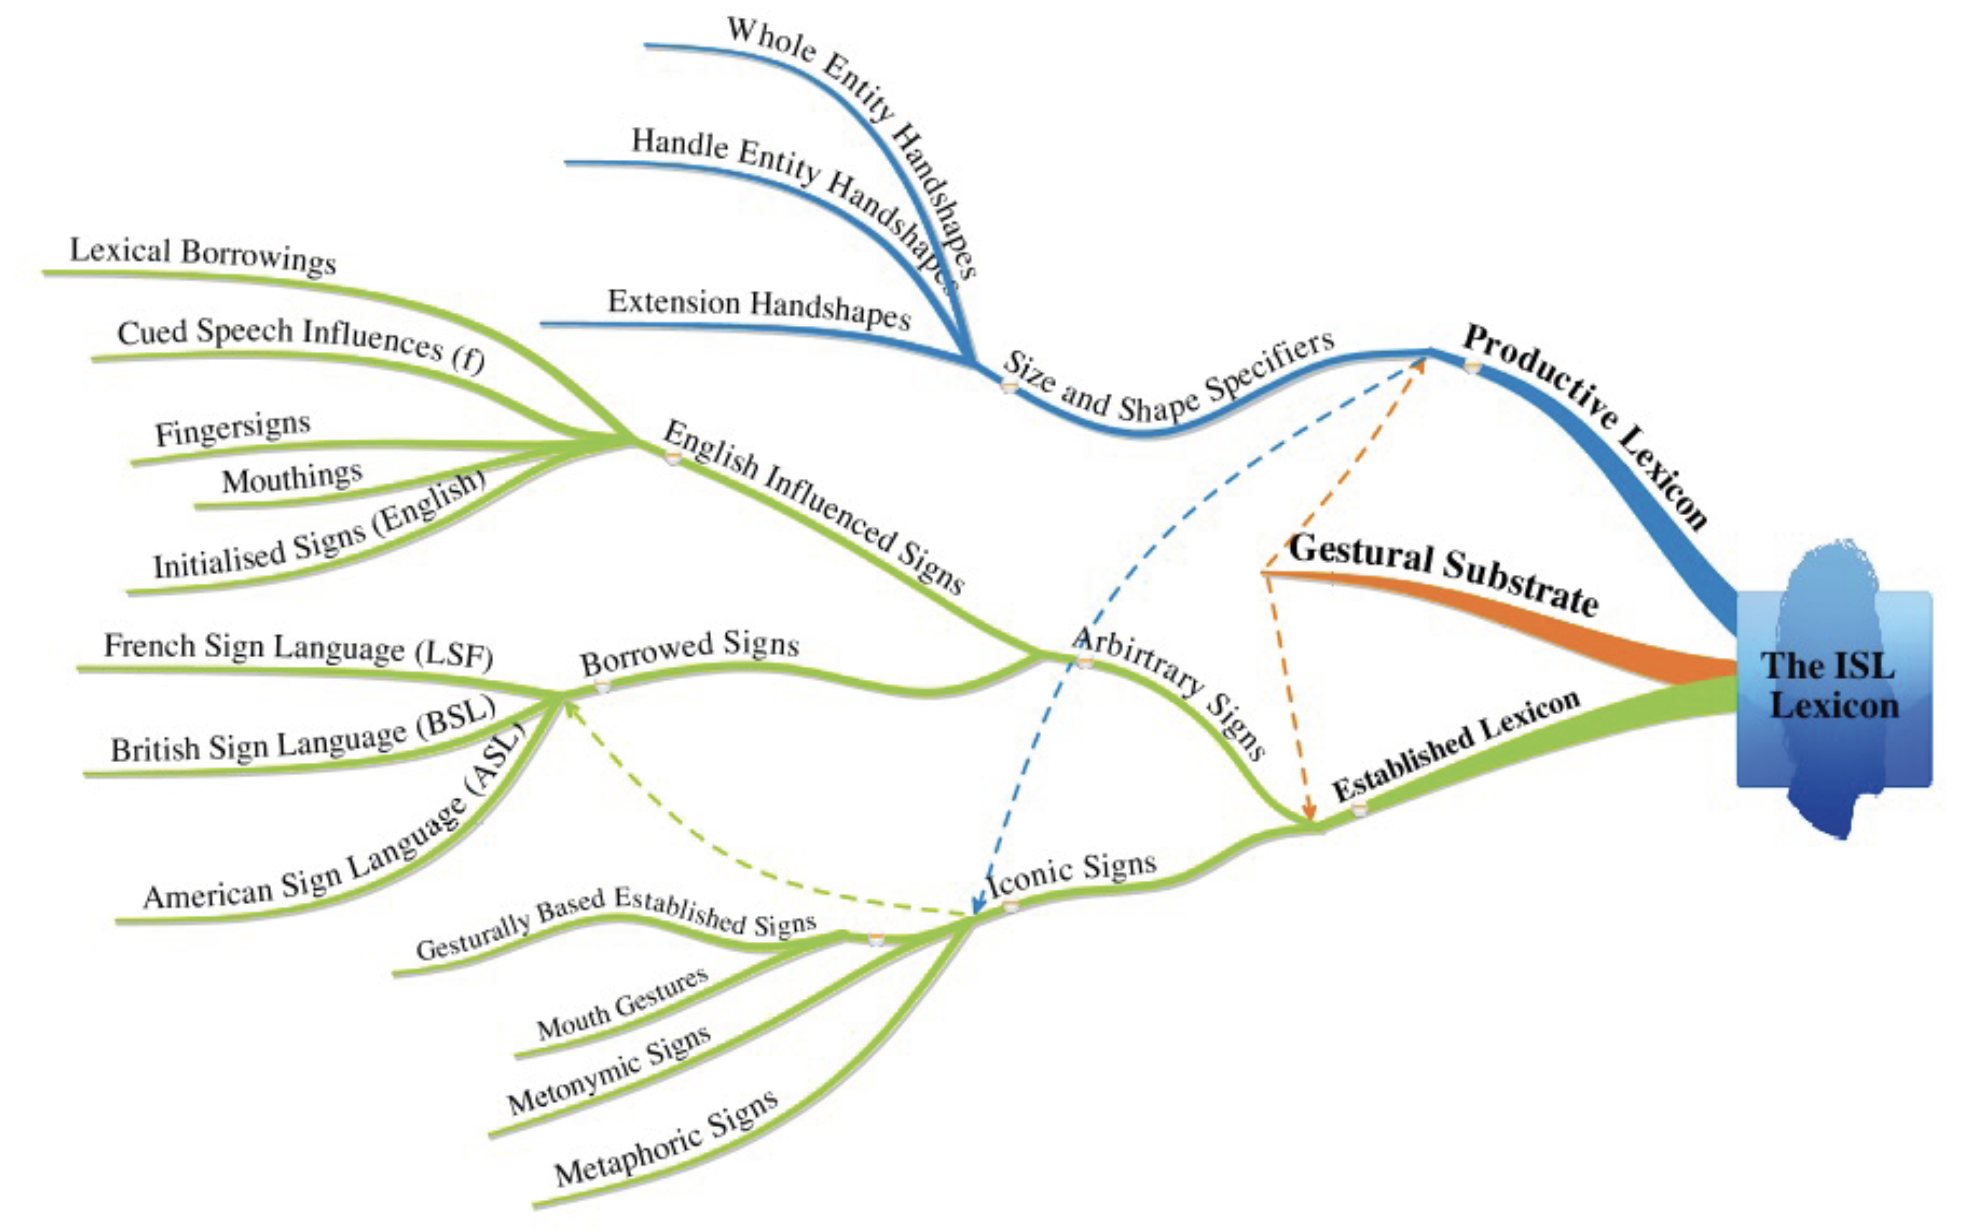
\includegraphics[width=\textwidth]{figures/lexicon.png}
\captionof{figure}{Extracted from \parencite{leeson2012}:127 Section 6.2, The ISL Lexicon}



\subsection{Stablished ISL Lexicon}

The established lexicon of ISL encompasses a variety of signs, both arbitrary and iconic. This includes signs that English has influenced, British Sign Language, French Sign Language, and more recently, American Sign Language. Certain iconic signs might have origins in gestures, often appearing as metonymic forms. Some of these signs are accompanied by mouth gestures, which have become conventionally linked to specific lexical items, particularly those associated with gender-specific concepts. (Leeson and Saeed, 2012)

\subsection{Productive ISL Lexicon}

In the productive lexicon, gesture is a fundamental building block for multiple functional elements. These elements have undergone standardisation, elevating them to a position of linguistic significance. Utilising size and shape specifiers, commonly called classifier handshapes, assumes a prominent role within this particular category. (Leeson and Saeed, 2012)









